\chapter{CMS Experiment}
\label{ch2}

\section{CMS detector}

The CMS is one of the four interactions points on the LHC. Its a cylindrical onion with several concentric layers this layers consist on different detectors made for detecting different particles, like the silicon tracker, the electromagnetic calorimeter, the hadron calorimeter the superconducting solenoid and the muon chamber. Its a cylindrical onion with several concentric layers.   \cite{CMS}

The Sylicon Tracker is composed of different substructures Its main purpose It's to reconstruct the trajectories of charged particles, in the point closest to the collision of the beams tis where the Sylicon Pixel Detector is located. %NEEDED\cite{CMS}

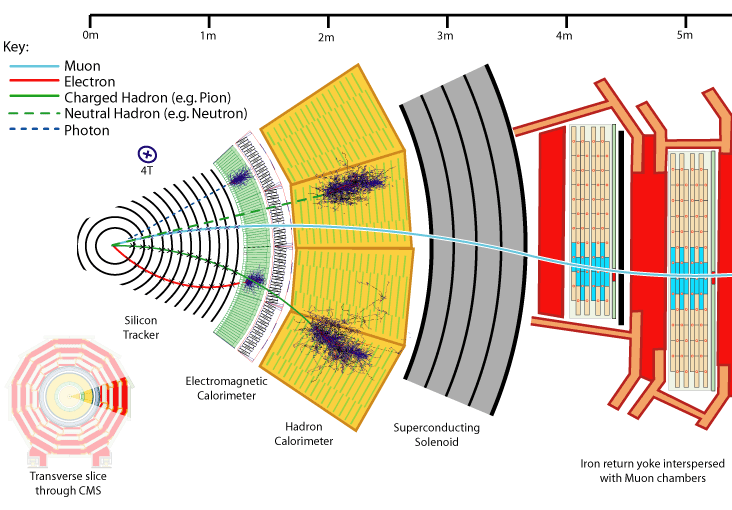
\includegraphics[scale=0.35]{cms.png}

The other parts of the detector are for locating different types of particles depending on their interactions , the electromagnetic calorimeter 


\section{Pixel Detector}

This is one of the detectors of the CMS \cite{pxd}

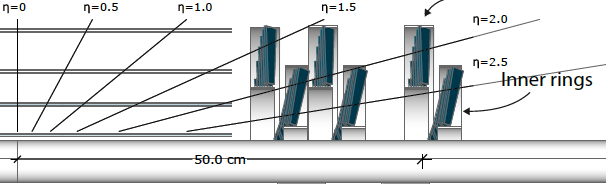
\includegraphics[scale=0.7]{pixeldetector.png}

\section{PCC}

The Pixel Cluster Counting (PCC) method


\section{Module Selection}



